\documentclass[tikz,border=6pt]{standalone}
\usepackage{fontspec}
\usepackage{newtxmath}
\usepackage{bm}
\usepackage{tikz}
\usetikzlibrary{calc,arrows.meta}

\definecolor{sfgreen}{RGB}{0,166,86}
\setmainfont{Times New Roman}

\begin{document}
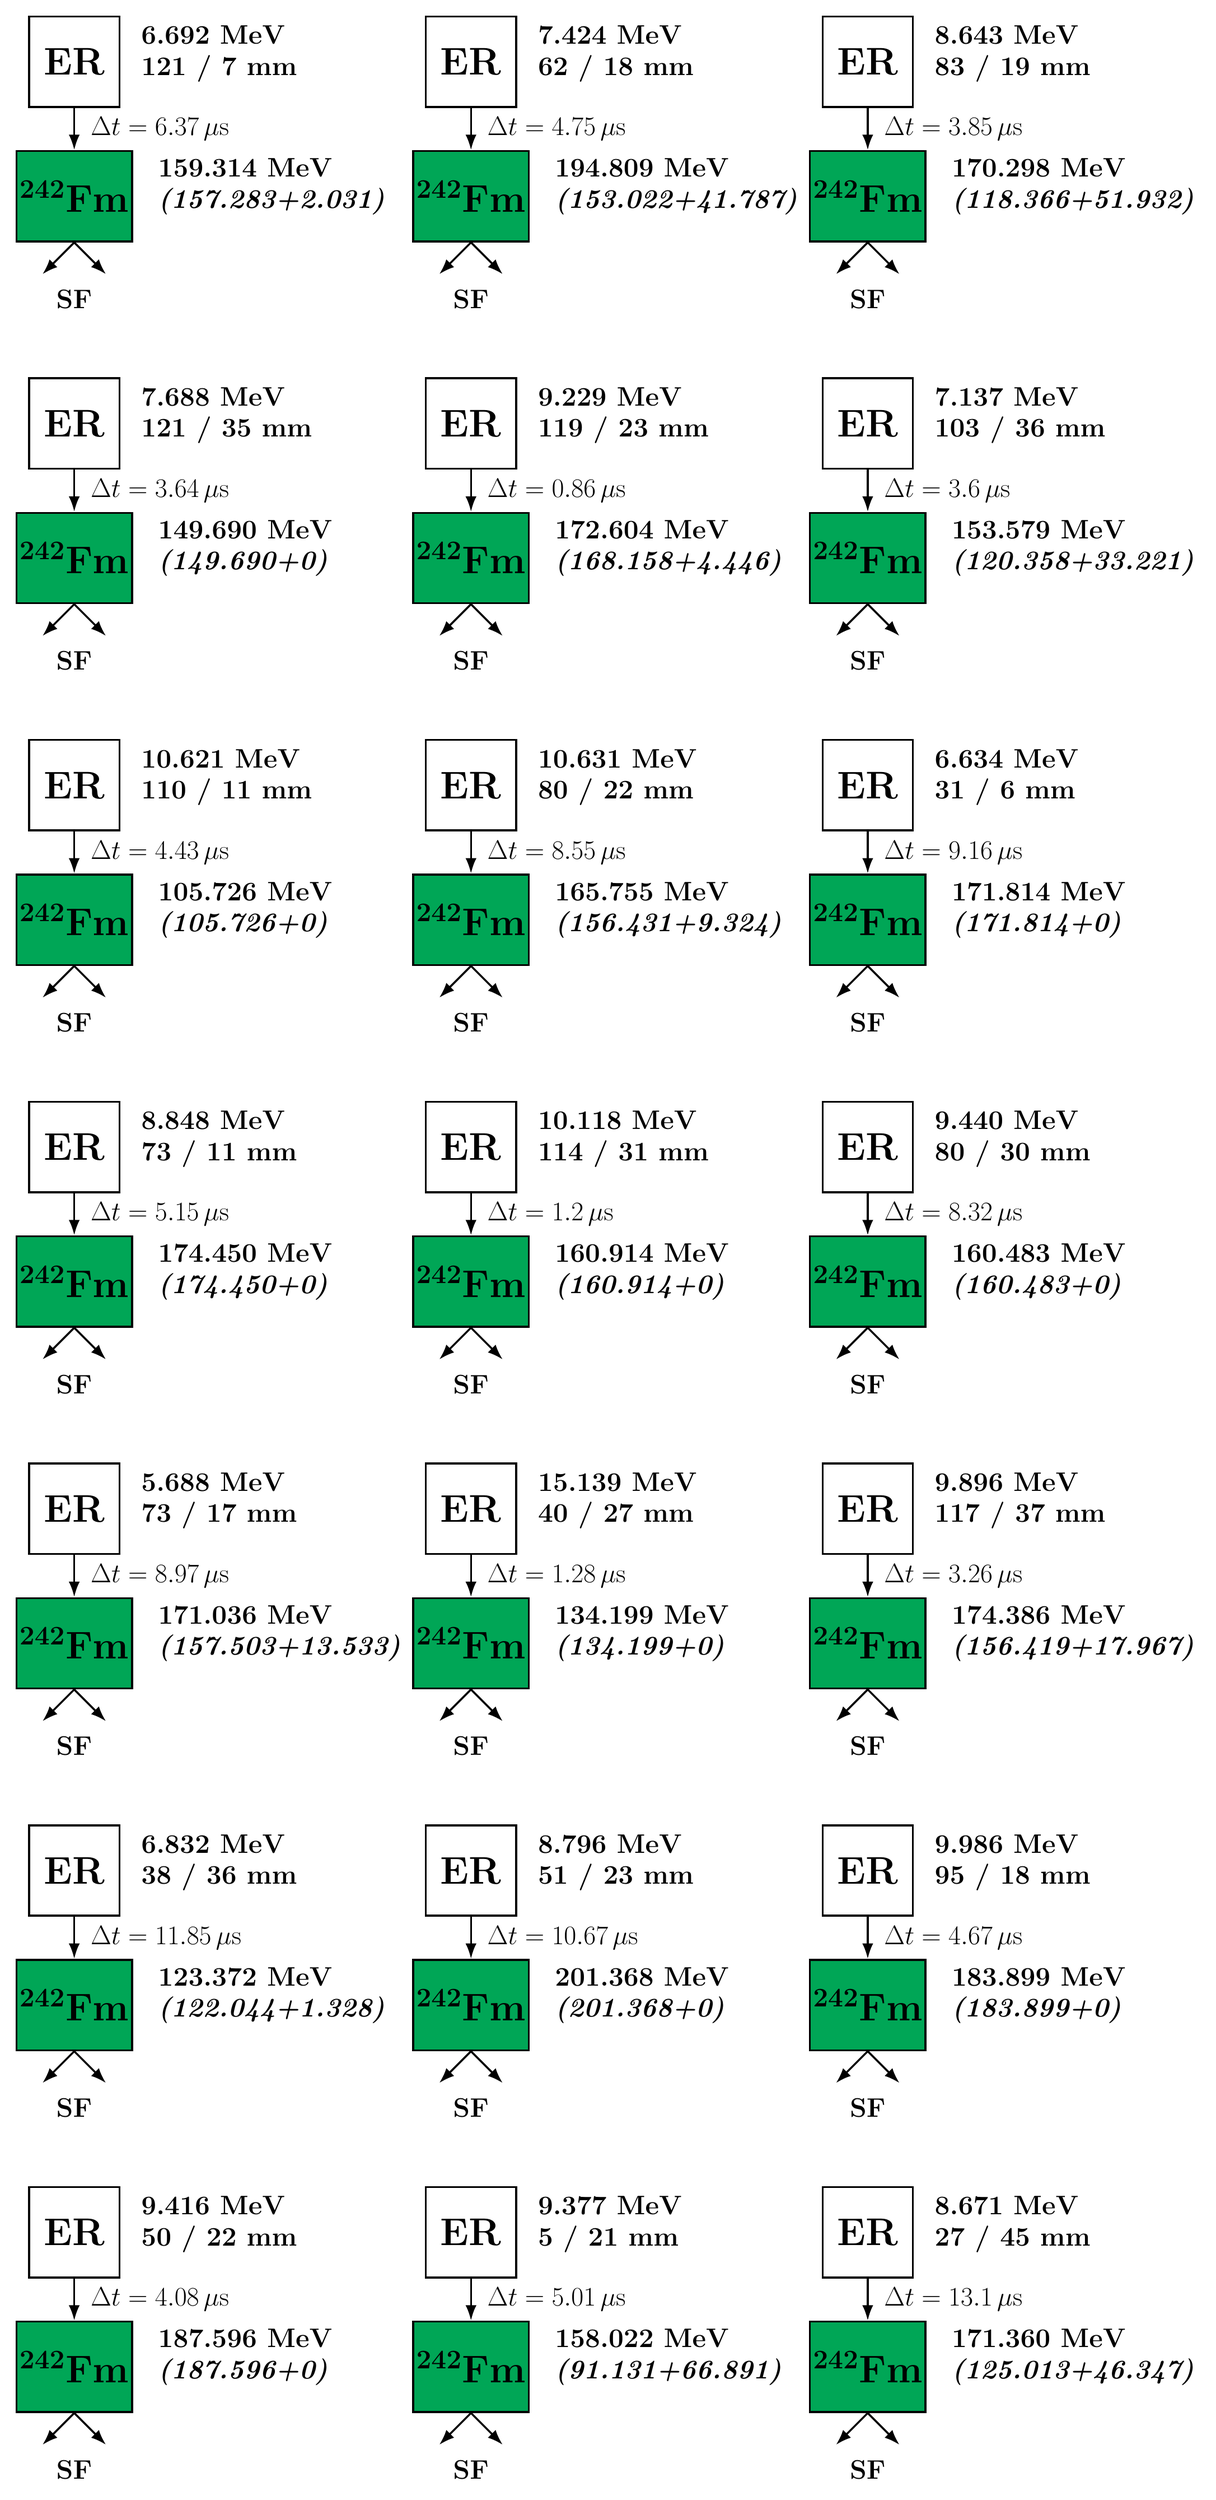
\begin{tikzpicture}[x=1cm,y=1cm]
\tikzset{
  nucW/.style={
    draw=black,
    line width=1.25pt,
    fill=white,
    minimum width=2.05cm,
    minimum height=2.05cm,
    align=center,
    inner sep=2pt,
    font=\bfseries\fontsize{24}{26}\selectfont
  },
  nucSF/.style={
    draw=black,
    line width=1.25pt,
    fill=sfgreen,
    minimum width=2.05cm,
    minimum height=2.05cm,
    align=center,
    inner sep=2pt,
    font=\bfseries\fontsize{24}{26}\selectfont
  },
  arr/.style={
    -{Latex[length=3.5mm,width=2.5mm]},
    line width=1.25pt,
    draw=black
  },
  datatxt/.style={
    font=\bfseries\fontsize{18}{20}\selectfont,
    text=black,
    align=left
  },
  sflabel/.style={
    font=\bfseries\fontsize{18}{20}\selectfont,
    text=black,
    align=center
  }
}

% Event 1
\begin{scope}[shift={(0.00,0.00)}]
  \node[nucW] (evt1implant) at (5.80,4.00) {ER};
  \node[nucSF] (evt1sf) at (5.80,0.95) {$\bm{{}^{242}\mathrm{Fm}}$};

  \draw[arr] (evt1implant.south) -- (evt1sf.north);
  \node[datatxt,anchor=west] at ($(evt1implant.south)!0.50!(evt1sf.north)+(0.25,0)$)
    {$\Delta t=6.37\,\mu\mathrm{s}$};
  \draw[arr] (evt1sf.south) -- ++(-0.72,-0.72);
  \draw[arr] (evt1sf.south) -- ++(0.72,-0.72);
  \node[sflabel,anchor=north] at ($(evt1sf.south)+(0,-0.95)$) {SF};

  \node[datatxt,anchor=west] at ($(evt1implant.east)+(0.35,0.18)$)
    {6.692 MeV\\121 / 7 mm};
  \node[datatxt,anchor=west] at ($(evt1sf.east)+(0.45,0.22)$)
    {159.314 MeV\\\textit{(157.283+2.031)}};
\end{scope}

% Event 2
\begin{scope}[shift={(9.00,0.00)}]
  \node[nucW] (evt2implant) at (5.80,4.00) {ER};
  \node[nucSF] (evt2sf) at (5.80,0.95) {$\bm{{}^{242}\mathrm{Fm}}$};

  \draw[arr] (evt2implant.south) -- (evt2sf.north);
  \node[datatxt,anchor=west] at ($(evt2implant.south)!0.50!(evt2sf.north)+(0.25,0)$)
    {$\Delta t=4.75\,\mu\mathrm{s}$};
  \draw[arr] (evt2sf.south) -- ++(-0.72,-0.72);
  \draw[arr] (evt2sf.south) -- ++(0.72,-0.72);
  \node[sflabel,anchor=north] at ($(evt2sf.south)+(0,-0.95)$) {SF};

  \node[datatxt,anchor=west] at ($(evt2implant.east)+(0.35,0.18)$)
    {7.424 MeV\\62 / 18 mm};
  \node[datatxt,anchor=west] at ($(evt2sf.east)+(0.45,0.22)$)
    {194.809 MeV\\\textit{(153.022+41.787)}};
\end{scope}

% Event 3
\begin{scope}[shift={(18.00,0.00)}]
  \node[nucW] (evt3implant) at (5.80,4.00) {ER};
  \node[nucSF] (evt3sf) at (5.80,0.95) {$\bm{{}^{242}\mathrm{Fm}}$};

  \draw[arr] (evt3implant.south) -- (evt3sf.north);
  \node[datatxt,anchor=west] at ($(evt3implant.south)!0.50!(evt3sf.north)+(0.25,0)$)
    {$\Delta t=3.85\,\mu\mathrm{s}$};
  \draw[arr] (evt3sf.south) -- ++(-0.72,-0.72);
  \draw[arr] (evt3sf.south) -- ++(0.72,-0.72);
  \node[sflabel,anchor=north] at ($(evt3sf.south)+(0,-0.95)$) {SF};

  \node[datatxt,anchor=west] at ($(evt3implant.east)+(0.35,0.18)$)
    {8.643 MeV\\83 / 19 mm};
  \node[datatxt,anchor=west] at ($(evt3sf.east)+(0.45,0.22)$)
    {170.298 MeV\\\textit{(118.366+51.932)}};
\end{scope}

% Event 4
\begin{scope}[shift={(0.00,-8.20)}]
  \node[nucW] (evt4implant) at (5.80,4.00) {ER};
  \node[nucSF] (evt4sf) at (5.80,0.95) {$\bm{{}^{242}\mathrm{Fm}}$};

  \draw[arr] (evt4implant.south) -- (evt4sf.north);
  \node[datatxt,anchor=west] at ($(evt4implant.south)!0.50!(evt4sf.north)+(0.25,0)$)
    {$\Delta t=3.64\,\mu\mathrm{s}$};
  \draw[arr] (evt4sf.south) -- ++(-0.72,-0.72);
  \draw[arr] (evt4sf.south) -- ++(0.72,-0.72);
  \node[sflabel,anchor=north] at ($(evt4sf.south)+(0,-0.95)$) {SF};

  \node[datatxt,anchor=west] at ($(evt4implant.east)+(0.35,0.18)$)
    {7.688 MeV\\121 / 35 mm};
  \node[datatxt,anchor=west] at ($(evt4sf.east)+(0.45,0.22)$)
    {149.690 MeV\\\textit{(149.690+0)}};
\end{scope}

% Event 5
\begin{scope}[shift={(9.00,-8.20)}]
  \node[nucW] (evt5implant) at (5.80,4.00) {ER};
  \node[nucSF] (evt5sf) at (5.80,0.95) {$\bm{{}^{242}\mathrm{Fm}}$};

  \draw[arr] (evt5implant.south) -- (evt5sf.north);
  \node[datatxt,anchor=west] at ($(evt5implant.south)!0.50!(evt5sf.north)+(0.25,0)$)
    {$\Delta t=0.86\,\mu\mathrm{s}$};
  \draw[arr] (evt5sf.south) -- ++(-0.72,-0.72);
  \draw[arr] (evt5sf.south) -- ++(0.72,-0.72);
  \node[sflabel,anchor=north] at ($(evt5sf.south)+(0,-0.95)$) {SF};

  \node[datatxt,anchor=west] at ($(evt5implant.east)+(0.35,0.18)$)
    {9.229 MeV\\119 / 23 mm};
  \node[datatxt,anchor=west] at ($(evt5sf.east)+(0.45,0.22)$)
    {172.604 MeV\\\textit{(168.158+4.446)}};
\end{scope}

% Event 6
\begin{scope}[shift={(18.00,-8.20)}]
  \node[nucW] (evt6implant) at (5.80,4.00) {ER};
  \node[nucSF] (evt6sf) at (5.80,0.95) {$\bm{{}^{242}\mathrm{Fm}}$};

  \draw[arr] (evt6implant.south) -- (evt6sf.north);
  \node[datatxt,anchor=west] at ($(evt6implant.south)!0.50!(evt6sf.north)+(0.25,0)$)
    {$\Delta t=3.6\,\mu\mathrm{s}$};
  \draw[arr] (evt6sf.south) -- ++(-0.72,-0.72);
  \draw[arr] (evt6sf.south) -- ++(0.72,-0.72);
  \node[sflabel,anchor=north] at ($(evt6sf.south)+(0,-0.95)$) {SF};

  \node[datatxt,anchor=west] at ($(evt6implant.east)+(0.35,0.18)$)
    {7.137 MeV\\103 / 36 mm};
  \node[datatxt,anchor=west] at ($(evt6sf.east)+(0.45,0.22)$)
    {153.579 MeV\\\textit{(120.358+33.221)}};
\end{scope}

% Event 7
\begin{scope}[shift={(0.00,-16.40)}]
  \node[nucW] (evt7implant) at (5.80,4.00) {ER};
  \node[nucSF] (evt7sf) at (5.80,0.95) {$\bm{{}^{242}\mathrm{Fm}}$};

  \draw[arr] (evt7implant.south) -- (evt7sf.north);
  \node[datatxt,anchor=west] at ($(evt7implant.south)!0.50!(evt7sf.north)+(0.25,0)$)
    {$\Delta t=4.43\,\mu\mathrm{s}$};
  \draw[arr] (evt7sf.south) -- ++(-0.72,-0.72);
  \draw[arr] (evt7sf.south) -- ++(0.72,-0.72);
  \node[sflabel,anchor=north] at ($(evt7sf.south)+(0,-0.95)$) {SF};

  \node[datatxt,anchor=west] at ($(evt7implant.east)+(0.35,0.18)$)
    {10.621 MeV\\110 / 11 mm};
  \node[datatxt,anchor=west] at ($(evt7sf.east)+(0.45,0.22)$)
    {105.726 MeV\\\textit{(105.726+0)}};
\end{scope}

% Event 8
\begin{scope}[shift={(9.00,-16.40)}]
  \node[nucW] (evt8implant) at (5.80,4.00) {ER};
  \node[nucSF] (evt8sf) at (5.80,0.95) {$\bm{{}^{242}\mathrm{Fm}}$};

  \draw[arr] (evt8implant.south) -- (evt8sf.north);
  \node[datatxt,anchor=west] at ($(evt8implant.south)!0.50!(evt8sf.north)+(0.25,0)$)
    {$\Delta t=8.55\,\mu\mathrm{s}$};
  \draw[arr] (evt8sf.south) -- ++(-0.72,-0.72);
  \draw[arr] (evt8sf.south) -- ++(0.72,-0.72);
  \node[sflabel,anchor=north] at ($(evt8sf.south)+(0,-0.95)$) {SF};

  \node[datatxt,anchor=west] at ($(evt8implant.east)+(0.35,0.18)$)
    {10.631 MeV\\80 / 22 mm};
  \node[datatxt,anchor=west] at ($(evt8sf.east)+(0.45,0.22)$)
    {165.755 MeV\\\textit{(156.431+9.324)}};
\end{scope}

% Event 9
\begin{scope}[shift={(18.00,-16.40)}]
  \node[nucW] (evt9implant) at (5.80,4.00) {ER};
  \node[nucSF] (evt9sf) at (5.80,0.95) {$\bm{{}^{242}\mathrm{Fm}}$};

  \draw[arr] (evt9implant.south) -- (evt9sf.north);
  \node[datatxt,anchor=west] at ($(evt9implant.south)!0.50!(evt9sf.north)+(0.25,0)$)
    {$\Delta t=9.16\,\mu\mathrm{s}$};
  \draw[arr] (evt9sf.south) -- ++(-0.72,-0.72);
  \draw[arr] (evt9sf.south) -- ++(0.72,-0.72);
  \node[sflabel,anchor=north] at ($(evt9sf.south)+(0,-0.95)$) {SF};

  \node[datatxt,anchor=west] at ($(evt9implant.east)+(0.35,0.18)$)
    {6.634 MeV\\31 / 6 mm};
  \node[datatxt,anchor=west] at ($(evt9sf.east)+(0.45,0.22)$)
    {171.814 MeV\\\textit{(171.814+0)}};
\end{scope}

% Event 10
\begin{scope}[shift={(0.00,-24.60)}]
  \node[nucW] (evt10implant) at (5.80,4.00) {ER};
  \node[nucSF] (evt10sf) at (5.80,0.95) {$\bm{{}^{242}\mathrm{Fm}}$};

  \draw[arr] (evt10implant.south) -- (evt10sf.north);
  \node[datatxt,anchor=west] at ($(evt10implant.south)!0.50!(evt10sf.north)+(0.25,0)$)
    {$\Delta t=5.15\,\mu\mathrm{s}$};
  \draw[arr] (evt10sf.south) -- ++(-0.72,-0.72);
  \draw[arr] (evt10sf.south) -- ++(0.72,-0.72);
  \node[sflabel,anchor=north] at ($(evt10sf.south)+(0,-0.95)$) {SF};

  \node[datatxt,anchor=west] at ($(evt10implant.east)+(0.35,0.18)$)
    {8.848 MeV\\73 / 11 mm};
  \node[datatxt,anchor=west] at ($(evt10sf.east)+(0.45,0.22)$)
    {174.450 MeV\\\textit{(174.450+0)}};
\end{scope}

% Event 11
\begin{scope}[shift={(9.00,-24.60)}]
  \node[nucW] (evt11implant) at (5.80,4.00) {ER};
  \node[nucSF] (evt11sf) at (5.80,0.95) {$\bm{{}^{242}\mathrm{Fm}}$};

  \draw[arr] (evt11implant.south) -- (evt11sf.north);
  \node[datatxt,anchor=west] at ($(evt11implant.south)!0.50!(evt11sf.north)+(0.25,0)$)
    {$\Delta t=1.2\,\mu\mathrm{s}$};
  \draw[arr] (evt11sf.south) -- ++(-0.72,-0.72);
  \draw[arr] (evt11sf.south) -- ++(0.72,-0.72);
  \node[sflabel,anchor=north] at ($(evt11sf.south)+(0,-0.95)$) {SF};

  \node[datatxt,anchor=west] at ($(evt11implant.east)+(0.35,0.18)$)
    {10.118 MeV\\114 / 31 mm};
  \node[datatxt,anchor=west] at ($(evt11sf.east)+(0.45,0.22)$)
    {160.914 MeV\\\textit{(160.914+0)}};
\end{scope}

% Event 12
\begin{scope}[shift={(18.00,-24.60)}]
  \node[nucW] (evt12implant) at (5.80,4.00) {ER};
  \node[nucSF] (evt12sf) at (5.80,0.95) {$\bm{{}^{242}\mathrm{Fm}}$};

  \draw[arr] (evt12implant.south) -- (evt12sf.north);
  \node[datatxt,anchor=west] at ($(evt12implant.south)!0.50!(evt12sf.north)+(0.25,0)$)
    {$\Delta t=8.32\,\mu\mathrm{s}$};
  \draw[arr] (evt12sf.south) -- ++(-0.72,-0.72);
  \draw[arr] (evt12sf.south) -- ++(0.72,-0.72);
  \node[sflabel,anchor=north] at ($(evt12sf.south)+(0,-0.95)$) {SF};

  \node[datatxt,anchor=west] at ($(evt12implant.east)+(0.35,0.18)$)
    {9.440 MeV\\80 / 30 mm};
  \node[datatxt,anchor=west] at ($(evt12sf.east)+(0.45,0.22)$)
    {160.483 MeV\\\textit{(160.483+0)}};
\end{scope}

% Event 13
\begin{scope}[shift={(0.00,-32.80)}]
  \node[nucW] (evt13implant) at (5.80,4.00) {ER};
  \node[nucSF] (evt13sf) at (5.80,0.95) {$\bm{{}^{242}\mathrm{Fm}}$};

  \draw[arr] (evt13implant.south) -- (evt13sf.north);
  \node[datatxt,anchor=west] at ($(evt13implant.south)!0.50!(evt13sf.north)+(0.25,0)$)
    {$\Delta t=8.97\,\mu\mathrm{s}$};
  \draw[arr] (evt13sf.south) -- ++(-0.72,-0.72);
  \draw[arr] (evt13sf.south) -- ++(0.72,-0.72);
  \node[sflabel,anchor=north] at ($(evt13sf.south)+(0,-0.95)$) {SF};

  \node[datatxt,anchor=west] at ($(evt13implant.east)+(0.35,0.18)$)
    {5.688 MeV\\73 / 17 mm};
  \node[datatxt,anchor=west] at ($(evt13sf.east)+(0.45,0.22)$)
    {171.036 MeV\\\textit{(157.503+13.533)}};
\end{scope}

% Event 14
\begin{scope}[shift={(9.00,-32.80)}]
  \node[nucW] (evt14implant) at (5.80,4.00) {ER};
  \node[nucSF] (evt14sf) at (5.80,0.95) {$\bm{{}^{242}\mathrm{Fm}}$};

  \draw[arr] (evt14implant.south) -- (evt14sf.north);
  \node[datatxt,anchor=west] at ($(evt14implant.south)!0.50!(evt14sf.north)+(0.25,0)$)
    {$\Delta t=1.28\,\mu\mathrm{s}$};
  \draw[arr] (evt14sf.south) -- ++(-0.72,-0.72);
  \draw[arr] (evt14sf.south) -- ++(0.72,-0.72);
  \node[sflabel,anchor=north] at ($(evt14sf.south)+(0,-0.95)$) {SF};

  \node[datatxt,anchor=west] at ($(evt14implant.east)+(0.35,0.18)$)
    {15.139 MeV\\40 / 27 mm};
  \node[datatxt,anchor=west] at ($(evt14sf.east)+(0.45,0.22)$)
    {134.199 MeV\\\textit{(134.199+0)}};
\end{scope}

% Event 15
\begin{scope}[shift={(18.00,-32.80)}]
  \node[nucW] (evt15implant) at (5.80,4.00) {ER};
  \node[nucSF] (evt15sf) at (5.80,0.95) {$\bm{{}^{242}\mathrm{Fm}}$};

  \draw[arr] (evt15implant.south) -- (evt15sf.north);
  \node[datatxt,anchor=west] at ($(evt15implant.south)!0.50!(evt15sf.north)+(0.25,0)$)
    {$\Delta t=3.26\,\mu\mathrm{s}$};
  \draw[arr] (evt15sf.south) -- ++(-0.72,-0.72);
  \draw[arr] (evt15sf.south) -- ++(0.72,-0.72);
  \node[sflabel,anchor=north] at ($(evt15sf.south)+(0,-0.95)$) {SF};

  \node[datatxt,anchor=west] at ($(evt15implant.east)+(0.35,0.18)$)
    {9.896 MeV\\117 / 37 mm};
  \node[datatxt,anchor=west] at ($(evt15sf.east)+(0.45,0.22)$)
    {174.386 MeV\\\textit{(156.419+17.967)}};
\end{scope}

% Event 16
\begin{scope}[shift={(0.00,-41.00)}]
  \node[nucW] (evt16implant) at (5.80,4.00) {ER};
  \node[nucSF] (evt16sf) at (5.80,0.95) {$\bm{{}^{242}\mathrm{Fm}}$};

  \draw[arr] (evt16implant.south) -- (evt16sf.north);
  \node[datatxt,anchor=west] at ($(evt16implant.south)!0.50!(evt16sf.north)+(0.25,0)$)
    {$\Delta t=11.85\,\mu\mathrm{s}$};
  \draw[arr] (evt16sf.south) -- ++(-0.72,-0.72);
  \draw[arr] (evt16sf.south) -- ++(0.72,-0.72);
  \node[sflabel,anchor=north] at ($(evt16sf.south)+(0,-0.95)$) {SF};

  \node[datatxt,anchor=west] at ($(evt16implant.east)+(0.35,0.18)$)
    {6.832 MeV\\38 / 36 mm};
  \node[datatxt,anchor=west] at ($(evt16sf.east)+(0.45,0.22)$)
    {123.372 MeV\\\textit{(122.044+1.328)}};
\end{scope}

% Event 17
\begin{scope}[shift={(9.00,-41.00)}]
  \node[nucW] (evt17implant) at (5.80,4.00) {ER};
  \node[nucSF] (evt17sf) at (5.80,0.95) {$\bm{{}^{242}\mathrm{Fm}}$};

  \draw[arr] (evt17implant.south) -- (evt17sf.north);
  \node[datatxt,anchor=west] at ($(evt17implant.south)!0.50!(evt17sf.north)+(0.25,0)$)
    {$\Delta t=10.67\,\mu\mathrm{s}$};
  \draw[arr] (evt17sf.south) -- ++(-0.72,-0.72);
  \draw[arr] (evt17sf.south) -- ++(0.72,-0.72);
  \node[sflabel,anchor=north] at ($(evt17sf.south)+(0,-0.95)$) {SF};

  \node[datatxt,anchor=west] at ($(evt17implant.east)+(0.35,0.18)$)
    {8.796 MeV\\51 / 23 mm};
  \node[datatxt,anchor=west] at ($(evt17sf.east)+(0.45,0.22)$)
    {201.368 MeV\\\textit{(201.368+0)}};
\end{scope}

% Event 18
\begin{scope}[shift={(18.00,-41.00)}]
  \node[nucW] (evt18implant) at (5.80,4.00) {ER};
  \node[nucSF] (evt18sf) at (5.80,0.95) {$\bm{{}^{242}\mathrm{Fm}}$};

  \draw[arr] (evt18implant.south) -- (evt18sf.north);
  \node[datatxt,anchor=west] at ($(evt18implant.south)!0.50!(evt18sf.north)+(0.25,0)$)
    {$\Delta t=4.67\,\mu\mathrm{s}$};
  \draw[arr] (evt18sf.south) -- ++(-0.72,-0.72);
  \draw[arr] (evt18sf.south) -- ++(0.72,-0.72);
  \node[sflabel,anchor=north] at ($(evt18sf.south)+(0,-0.95)$) {SF};

  \node[datatxt,anchor=west] at ($(evt18implant.east)+(0.35,0.18)$)
    {9.986 MeV\\95 / 18 mm};
  \node[datatxt,anchor=west] at ($(evt18sf.east)+(0.45,0.22)$)
    {183.899 MeV\\\textit{(183.899+0)}};
\end{scope}

% Event 19
\begin{scope}[shift={(0.00,-49.20)}]
  \node[nucW] (evt19implant) at (5.80,4.00) {ER};
  \node[nucSF] (evt19sf) at (5.80,0.95) {$\bm{{}^{242}\mathrm{Fm}}$};

  \draw[arr] (evt19implant.south) -- (evt19sf.north);
  \node[datatxt,anchor=west] at ($(evt19implant.south)!0.50!(evt19sf.north)+(0.25,0)$)
    {$\Delta t=4.08\,\mu\mathrm{s}$};
  \draw[arr] (evt19sf.south) -- ++(-0.72,-0.72);
  \draw[arr] (evt19sf.south) -- ++(0.72,-0.72);
  \node[sflabel,anchor=north] at ($(evt19sf.south)+(0,-0.95)$) {SF};

  \node[datatxt,anchor=west] at ($(evt19implant.east)+(0.35,0.18)$)
    {9.416 MeV\\50 / 22 mm};
  \node[datatxt,anchor=west] at ($(evt19sf.east)+(0.45,0.22)$)
    {187.596 MeV\\\textit{(187.596+0)}};
\end{scope}

% Event 20
\begin{scope}[shift={(9.00,-49.20)}]
  \node[nucW] (evt20implant) at (5.80,4.00) {ER};
  \node[nucSF] (evt20sf) at (5.80,0.95) {$\bm{{}^{242}\mathrm{Fm}}$};

  \draw[arr] (evt20implant.south) -- (evt20sf.north);
  \node[datatxt,anchor=west] at ($(evt20implant.south)!0.50!(evt20sf.north)+(0.25,0)$)
    {$\Delta t=5.01\,\mu\mathrm{s}$};
  \draw[arr] (evt20sf.south) -- ++(-0.72,-0.72);
  \draw[arr] (evt20sf.south) -- ++(0.72,-0.72);
  \node[sflabel,anchor=north] at ($(evt20sf.south)+(0,-0.95)$) {SF};

  \node[datatxt,anchor=west] at ($(evt20implant.east)+(0.35,0.18)$)
    {9.377 MeV\\5 / 21 mm};
  \node[datatxt,anchor=west] at ($(evt20sf.east)+(0.45,0.22)$)
    {158.022 MeV\\\textit{(91.131+66.891)}};
\end{scope}

% Event 21
\begin{scope}[shift={(18.00,-49.20)}]
  \node[nucW] (evt21implant) at (5.80,4.00) {ER};
  \node[nucSF] (evt21sf) at (5.80,0.95) {$\bm{{}^{242}\mathrm{Fm}}$};

  \draw[arr] (evt21implant.south) -- (evt21sf.north);
  \node[datatxt,anchor=west] at ($(evt21implant.south)!0.50!(evt21sf.north)+(0.25,0)$)
    {$\Delta t=13.1\,\mu\mathrm{s}$};
  \draw[arr] (evt21sf.south) -- ++(-0.72,-0.72);
  \draw[arr] (evt21sf.south) -- ++(0.72,-0.72);
  \node[sflabel,anchor=north] at ($(evt21sf.south)+(0,-0.95)$) {SF};

  \node[datatxt,anchor=west] at ($(evt21implant.east)+(0.35,0.18)$)
    {8.671 MeV\\27 / 45 mm};
  \node[datatxt,anchor=west] at ($(evt21sf.east)+(0.45,0.22)$)
    {171.360 MeV\\\textit{(125.013+46.347)}};
\end{scope}

\end{tikzpicture}
\end{document}
